% Por hacer:
% Dibujar el grafo de la fiesta del profesor McBrain

\section{Grafos}

Los grafos son objetos que resultan bastante útiles en las matemáticas discretas. Su nombre se deriva del hecho de que se pueden tomar en cuenta como una forma de notación gráfica o pictórica, y en este único aspecto recuerdan a los gráficos de las funciones que se ven en matemáticas básicas. Pero estos grafos no tienen tanto que ver con funciones, sino más con lo que conocemos como "redes".

\begin{defn}
    Un \ul{grafo} $G$ consiste de un conjunto finito $V$, cuyos miembros son llamados vértices, y un conjunto $L$, formado por todos los subconjuntos de $V$ de dos elementos\marginfootnote{En notación de teoría de conjuntos, tendríamos:
    \[
    X^{[2]} = \{ A \subset X : |A| = 2 \}
    \]} cuyos miembros se llaman \ul{lados}. Escribimos $G = (V,L)$ y decimos que $V$ es el \ul{conjunto de vértices} y $L$ el \ul{conjunto de lados}.
\end{defn}

\begin{ejem}\label{ej:grafo}
    Un ejemplo de un grafo $G = (V,L)$ está dado por los conjuntos
    
    \[
    V = \{ a, b, c, d, z \}, \quad L = \{ \{a,b\}, \{a,d\}, \{b,z\}, \{c,d\}, \{d,z\} \}
    \]
    
    sin embargo, este ejemplo es más intuitivo cuando dibujamos el grafo:
    
    \begin{center}
        \begin{tikzpicture}[scale=1.20]
            \SetGraphUnit{2}
            \Vertices{circle}{b,a,z,d,c}
            \Edges(a,b,z,d,a,d,c)
        \end{tikzpicture}
    \end{center}
\end{ejem}

\begin{notn}
    Al hablar de grafos, vamos a tener las siguientes convenciones:
    \begin{enumerate}
        \item Si tenemos un lado $\{x,y\} \in L$, entonces lo escribiremos como $xy \in L$.
        \item En este caso decimos que $x$ es \ul{vecino} de $y$ o que $x$ está \ul{conectado} a $y$.
        \item El \ul{conjunto de vecinos} de $x$ lo denotaremos por $N(x) = \{ y \in V : xy \in L \}$.
    \end{enumerate}
\end{notn}

\begin{ejem}
    El profesor McBrain y su esposa April hacen una fiesta en la que se encuentran otras cuatro parejas casadas. Algunas parejas se saludan cuando se encuentran, pero obviamente ninguna se saluda entre si. Al final de la fiesta, el profesor le pregunta a todos con cuántas personas se han saludado, y recibe nueve preguntas distintas. ¿Cuántas personas saludó April?:
\end{ejem}

    \begin{proof}[Respuesta]
    Primero, construímos un grafo cuyos vértices son las personas que están en la fiesta, y colocamos un lado $xy$ si $x$ e $y$ se saludaron. Como hay nueve personas además del profesor McBrain, y la máxima cantidad de apretones de manos que puede recibir una persona es 8, se sigue que las nueve respuestas recibidas han de ser 0, 1, 2, 3, 4, 5, 6, 7, 8. Denotamos cada vértice por estos números y con $M$ al profesor McBrain.
    
    \begin{figure}[h]
        \centering
        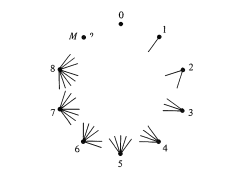
\includegraphics[scale=0.9]{img/Mcbrain.png}
        \caption{Representación pictórica de la fiesta y las respuestas recibidas por el profesor. No construí el grafo en latex porque soy bien neófito con tkz-graph y me dio flojera pasar dos horas leyendo la documentación para ver cómo. Es probable que en un futuro regrese a estas notas y lo haga, pero por ahora hay que conformarse con esta captura sacada del libro.}
    \end{figure}
    
    Ahora, el vértice 8 está unido a todos los demás puntos, excepto uno solo, el cual ha de representar a la pareja de 8. Este punto es cero. Continuando con este argumento, el 7 está unido con todos los puntos excepto 0 y 1 (este último ya está unido con 8), por lo que debe ser pareja de 1. De esta misma manera, concluimos que 6 y 2, y 3 y 5 son parejas. Únicamente queda 4, quien debe ser April.
    
    De esta forma, hemos concluído que April saludó a 4 personas.
\end{proof}

Otra forma de representar los grafos es a través de una \ul{lista de adyacencia}, la cual nos permite tener a los grafos como una lista o tabla. Para ello, diremos que dos vértices $x$ e $y$ son \ul{adyacentes} cuando $xy$ es un lado. Entonces, en la lista cada vértice $v$ encabezará una lista con todos los vértices adyacentes a $v$. El grafo del ejemplo \ref{ej:grafo}, tiene la siguiente lista de adyacencia:

\begin{center}
    \begin{tabular}{ccccc}
        $a$ & $b$ & $c$ & $d$ & $z$ \\ \toprule
        $b$ & $a$ & $d$ & $a$ & $b$ \\
        $d$ & $z$ &     & $c$ & $d$ \\
            &     &     & $z$ &     
    \end{tabular}
\end{center}

A su vez, también podemos establecer la \ul{matriz de adyacencia} $A = (a_{ij})$ de un grafo, donde tendremos que

\[ a_{ij} =
\begin{cases}
    1 \text{ si } v_iv_j \in L \\
    1 \text{ si no}
\end{cases}
\]

Para el mismo ejemplo, tenemos que la matriz de adyacencia es

\[
\begin{matrix}
        & $a$ & $b$ & $c$ & $d$ & $z$ \\
    $a$ &  0  &  1  &  0  &  1  &  0  \\
    $b$ &  1  &  0  &  0  &  0  &  1  \\
    $c$ &  0  &  0  &  0  &  1  &  0  \\
    $d$ &  1  &  0  &  1  &  0  &  1  \\
    $z$ &  0  &  1  &  0  &  1  &  0
\end{matrix}
\]

Nótese que si se cambia el orden de los vértices, tenemos otra matriz de adyacencia, por lo que usualmente se habla de \textbf{una} matriz de adyacencia.

\subsection{Isomorfismo de grafos}

Ahora pasaremos a contestar la pregunta de qué queremos decir cuando decimos que dos grafos son el mismo.

La característica principal de un grafo es la manera en que los vértices están emparejados por los lados. De aquí, tenemos la siguiente definición.

\begin{defn}
    Se dice que dos grafos $G_1$, $G_2$ son \ul{isomorfos} si se puede hacer una biyección $f$ del conjunto de vértices de $G_1$ al conjunto de vértices de $G_2$ tal que $xy \in L_1 \iff f(x)f(y) \in L_2$. Se dice que la biyección $f$ es un \ul{isomorfismo}.
\end{defn}

\begin{ejem}
    A continuación, un ejemplo de lo que queremos decir con isomorfismo de grafos:
    
    \begin{figure}
        \begin{subfigure}[b]{.5\textwidth}
            \centering
            \begin{tikzpicture}
                \GraphInit[vstyle=Normal]
                \SetGraphUnit{2}
                \begin{scope}[rotate=-135]
                \Vertices{circle}{d, c, b, a}
                \end{scope}
                \Edges(a, b, c, d, a, d, b)
            \end{tikzpicture}
            \caption{$G_1$}
        \end{subfigure}
        \hfill
        \begin{subfigure}[b]{.5\textwidth}
            \centering
            \begin{tikzpicture}[scale=0.7]
                \SetGraphUnit{2}
                \GraphInit[vstyle=Normal]
                \Vertex{v}
                \NOEA(v){w} \SOEA(w){u} \NO(w){t}
                \Edges(v, u, t, v, w, t, w, u)
            \end{tikzpicture}
            \caption{$G_2$}
        \end{subfigure}
        \caption{$G_1$ y $G_2$ son isomorfos.} 
    \end{figure}
\end{ejem}

\begin{teo}
    Si $G$ y $H$ son isomorfos mediante $\Phi: V(G) \rightarrow V(H)$, entonces $\forall x \in V(G)$, tenemos que $d(\Phi(x)) = d(x)$. El recíproco no es cierto.
\end{teo}

\begin{proof}
    La demostración es trivial: Sale por el hecho de que $xy \in L_1 \iff \Phi(x)\Phi(y) \in L_2$, por lo que cada vértice de $L_1$ estará conectado a la misma cantidad de vértices que su contraparte de $L_2$.
    
    El ejercicio 8.2.1 del Biggs es un contraejemplo del recíproco.
\end{proof}

\subsection{Grado (Valencia)}

\begin{defn}
    El \ul{grado} de un vértice $x$ en un grafo $G=(V,L)$ es el número de vecinos de $x$. Usaremos la notación $d(x)$ para referirnos al grado de $x$, entonces de manera formal,
    
    \[
    d(x) = |N(x)| \quad \text{donde} \quad N(x) = \{ y \in V : xy \in L \}
    \]
\end{defn}

\begin{teo}\label{teo:prehistorico}
    La suma de los grados de cada vértice $x \in V$ de un grafo $G = (V,L)$ es igual al doble del número de lados:
    
    \[
    \sum_{x \in V} d(x) = 2|L|
    \]
\end{teo}

\begin{proof}
    Para cada vértice, tendremos que se contará el grado, es decir cuántos vecinos tiene dicho vértice. Esto es lo mismo que decir que contaremos cuántos lados contienen al vértice. Como esto se hace para cada vértice, se contarán todos los lados dos veces: Una vez cuando estemos tomando en cuenta cualquier vértice y otra cuando estemos tomando en cuenta su vecino.
\end{proof}

Consideremos ahora

\[
\sum_{\substack{x \in V \\ d(x) \text{ es par}}} d(x) + \sum_{\substack{x \in V \\ d(x) \text{ es impar}}} d(x) = 2|L|
\]

entonces de aquí se desprende que hay una cantidad par de vértices impares.

Enunciamos el siguiente teorema.

\begin{teo}
    En todo grafo $G$ hay una cantidad par de vértices impares.
\end{teo}

\begin{defn}
    Un grafo en el cual todos los vértices tienen el mismo grado $k$, se le llama \ul{$k$-regular}. En este caso, el resultado del teorema \ref{teo:prehistorico} es
    
    \[
    k|V| = 2|L|
    \]
\end{defn}

Muchos de los grafos que veremos son regulares, como por ejemplo:

\begin{enumerate}
    \item $K_n$, el \textbf{grafo completo} este está definido de la siguiente manera:
    
    \[
    K_n = G(\{1,2, \dots, n\}, \{1,2, \dots, n\}^{[2]})
    \]
    
    Estos grafos son regulares, con grado $n-1$, y tienen $n(n-1)/2$ vértices\marginfootnote{Esta es una demostración de geometría, se puede hacer como ejercicio.}.Por ejemplo, si queremos representar $K_5$, tenemos:
    
    \begin{figure}[h]
        \centering
        \begin{tikzpicture}[scale=0.4]
            \GraphInit[vstyle=Normal]
            \grComplete[RA=5]{5}
            \end{tikzpicture}
        \caption{Grafo completo $K_5$.}
    \end{figure}
    
    \item En geometría se definen los polígonos de $n$ lados, los cuales corresponden en teoría de grafos a los \textbf{grafos cíclicos} $C_n$. Formalmente, podemos decir que el conjunto de vértices de $C_n$ es $\Z_n$, donde los vértices $i$ y $j$ se unen con un lado si $j = i + 1$ en $\Z_n$. Claramente, $C_n$ es un grafo regular con grado 2, dado $n \geq 3$. Un ejemplo podría ser el siguiente grafo cíclico:
    
    \begin{figure}[h]
        \centering
        \begin{tikzpicture}[scale=0.3]
            \GraphInit[vstyle=Normal]
            \grEmptyCycle[RA=5,prefix=a]{8}%
            \EdgeInGraphLoop{a}{8}
        \end{tikzpicture}
        \caption{Grafo cíclico $C_8$.}
    \end{figure}
\end{enumerate}